\documentclass[a4paper,11pt]{article}

\usepackage[margin=2.5cm]{geometry}
\usepackage{listings}
\usepackage{xcolor}
\usepackage{hyperref}
\usepackage{tikz}
\usetikzlibrary{chains,arrows.meta,shapes.misc,calc}

\hypersetup{colorlinks=true,linkcolor=blue!60!black,urlcolor=blue!60!black}

% -- EBNF listing style --
\lstdefinelanguage{EBNF}{
  morekeywords={},
  morecomment=[s]{/*}{*/},
  morestring=[b]',
  literate=
    {::=}{{{\color{red!70!black}::=}}}3
    {|}{{{\color{red!70!black}|}}}1
    {(}{{{\color{gray!70!black}(}}}1
    {)}{{{\color{gray!70!black})}}}1
    {*}{{{\color{red!70!black}*}}}1
    {+}{{{\color{red!70!black}+}}}1
    {?}{{{\color{red!70!black}?}}}1,
}

\lstset{
  language=EBNF,
  basicstyle=\ttfamily\small,
  keywordstyle=\color{black},
  commentstyle=\color{green!50!black}\itshape,
  stringstyle=\color{blue!70!black},
  showstringspaces=false,
  breaklines=true,
  frame=none,
  columns=fullflexible,
  keepspaces=true,
  tabsize=4,
  aboveskip=0.5em,
  belowskip=0.5em,
}

% -- Railroad diagram macros via TikZ --
\tikzset{
  rr terminal/.style={
    rounded rectangle,
    minimum height=6mm,
    minimum width=10mm,
    very thick,
    draw=black!50,
    top color=white,
    bottom color=black!15,
    font=\ttfamily\small,
    inner sep=3pt,
  },
  rr nonterminal/.style={
    rectangle,
    minimum height=6mm,
    minimum width=10mm,
    very thick,
    draw=red!50!black!50,
    top color=white,
    bottom color=red!50!black!15,
    font=\itshape\small,
    inner sep=3pt,
  },
  rr point/.style={circle, inner sep=0pt, minimum size=0pt, fill=black},
  rr arrow/.style={-{Stealth[length=3pt]}, thick},
  rr line/.style={thick},
}

% Railroad: terminal node
\newcommand{\rrT}[1]{\node[rr terminal]{#1};}
% Railroad: nonterminal node
\newcommand{\rrN}[1]{\node[rr nonterminal]{#1};}

\title{\textbf{Orchfile Grammar Reference}}
\author{Orchfile Specification}
\date{}

\begin{document}
\maketitle
\thispagestyle{empty}

\noindent
This document contains the formal grammar for Orchfile in W3C EBNF notation,
followed by railroad (syntax) diagrams for the key production rules.
The canonical source is \texttt{grammar.ebnf} in the repository root.

\tableofcontents
\newpage

% ============================================================================
\section{EBNF Grammar}
% ============================================================================

\subsection{Document Structure}

\begin{lstlisting}
orchfile     ::= ( line newline )*
line         ::= blank | comment | arg | service_decl | directive
blank        ::= ws*
comment      ::= ws* '#' any*
\end{lstlisting}

\subsection{Top-level Declarations}

\begin{lstlisting}
arg          ::= 'ARG' ws identifier '=' value
service_decl ::= 'SERVICE' ws service_name
\end{lstlisting}

\subsection{Directives}

\begin{lstlisting}
directive    ::= mode_directive
               | container_directive
               | host_directive
               | common_directive
               | clear_directive
\end{lstlisting}

\subsubsection{Overlay Composition}

\begin{lstlisting}
clear_directive
             ::= 'CLEAR' ws clearable_target

clearable_target
             ::= 'ENV' | 'ENV_FILE' | 'PUBLISH' | 'VOLUME'
               | 'REQUIRES' | 'AFTER'
\end{lstlisting}

\subsubsection{Execution Mode (mutually exclusive per service)}

\begin{lstlisting}
mode_directive
             ::= 'FROM' ws image_ref
               | 'RUN' ws command_string
\end{lstlisting}

\subsubsection{Container-only Directives}

\begin{lstlisting}
container_directive
             ::= 'ENTRYPOINT' ws command_string
               | 'CMD' ws command_string
               | 'PUBLISH' ws port ':' port
               | 'VOLUME' ws volume_source ':' path
\end{lstlisting}

\subsubsection{Host-only Directives}

\begin{lstlisting}
host_directive
             ::= 'USER' ws identifier
               | 'STOP' ws command_string
               | 'RELOAD' ws command_string
\end{lstlisting}

\subsubsection{Common Directives}

\begin{lstlisting}
common_directive
             ::= env_directive
               | dependency_directive
               | health_directive
               | lifecycle_directive
               | restart_directive
               | timeout_directive
               | resource_directive
               | logging_directive

env_directive
             ::= 'WORKDIR' ws path
               | 'ENV' ws env_key '=' value
               | 'ENV_FILE' ws path

dependency_directive
             ::= 'REQUIRES' ws service_name ( ws service_name )*
               | 'AFTER' ws service_name ( ws service_name )*

health_directive
             ::= 'HEALTHCHECK' ws ( url | command_string )
               | 'READINESS_TIMEOUT' ws duration

lifecycle_directive
             ::= 'ONESHOT' ws bool
               | 'DISABLED' ws bool
               | 'RECREATE' ws recreate_policy

restart_directive
             ::= 'RESTART' ws restart_policy
               | 'RESTART_DELAY' ws duration
               | 'START_LIMIT_BURST' ws integer
               | 'START_LIMIT_INTERVAL' ws duration

timeout_directive
             ::= 'TIMEOUT_START' ws duration
               | 'TIMEOUT_STOP' ws duration

resource_directive
             ::= 'MEMORY' ws memory_size
               | 'CPUS' ws number
               | 'CPU_QUOTA' ws percentage
               | 'LIMIT_NOFILE' ws integer
               | 'LIMIT_NPROC' ws integer
               | 'TASKS_MAX' ws integer
               | 'IO_WEIGHT' ws integer     /* 10-1000 */

logging_directive
             ::= 'STDOUT' ws path
               | 'STDERR' ws path
\end{lstlisting}

\subsection{Terminals}

\begin{lstlisting}
service_name    ::= letter ( letter | digit | '-' )*  /* max 63 chars */
identifier      ::= letter ( letter | digit | '_' )*
env_key         ::= ( letter | '_' ) ( letter | digit | '_' )*

image_ref       ::= ( any - newline )+
command_string  ::= ( any - newline )+
path            ::= ( any - newline )+
value           ::= ( any - newline )*
url             ::= ( 'http://' | 'https://' ) ( any - newline )+

var_ref         ::= '${' identifier '}'

bool            ::= 'true' | 'false'
restart_policy  ::= 'no' | 'always' | 'on-failure'
recreate_policy ::= 'always' | 'never'

duration        ::= integer ( 's' | 'm' )
memory_size     ::= integer ( 'K' | 'M' | 'G' )
percentage      ::= integer '%'
number          ::= integer ( '.' digit+ )?
integer         ::= digit+
port            ::= digit+                             /* 1-65535 */

letter          ::= [a-z]
digit           ::= [0-9]
ws              ::= [ \t]+
newline         ::= \n
any             ::= [U+0020-U+FFFF]
\end{lstlisting}

\medskip
\noindent
\textbf{Note:} \texttt{var\_ref} (\texttt{\$\{name\}}) may appear within any
\texttt{value}, \texttt{path}, \texttt{image\_ref}, or \texttt{command\_string}.
Variable expansion is performed at parse time using resolved ARG values.
Unresolved references to built-in variables (e.g.\ \texttt{\$\{ORCH\_PROJECT\}})
are preserved for runtime resolution.

% ============================================================================
\newpage
\section{Railroad Diagrams}
% ============================================================================

The following diagrams visualize the key production rules.
Rounded boxes are \textit{terminals} (literal text), rectangular boxes are
\textit{non-terminals} (references to other rules).

\bigskip

% --- orchfile ---
\noindent\textbf{orchfile}
\medskip

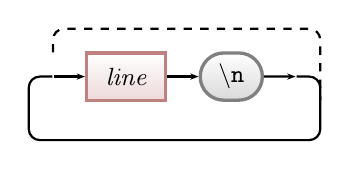
\begin{tikzpicture}[
  start chain=going right,
  node distance=5mm and 4mm,
  every node/.style={on chain},
  every join/.style={rr arrow},
]
  \node[rr point] (start) {};
  \node[rr nonterminal,join] {line};
  \node[rr terminal,join] {\textbackslash n};
  \node[rr point,join] (end) {};
  \draw[rr line,rounded corners] (end.east) -- ++(0.3,0) |- ([yshift=-8mm]start.south) -| ([xshift=-3mm]start.west) -- (start.west);
  \draw[rr line,dashed,rounded corners] (start.north) ++ (0,3mm) -- ++(0,3mm) -| ([xshift=3mm]end.east) -- ++ (0,-3mm);
\end{tikzpicture}

\bigskip

% --- arg ---
\noindent\textbf{arg}
\medskip

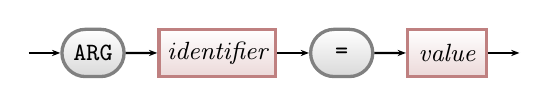
\begin{tikzpicture}[
  start chain=going right,
  node distance=5mm and 4mm,
  every node/.style={on chain},
  every join/.style={rr arrow},
]
  \node[rr point] {};
  \node[rr terminal,join] {ARG};
  \node[rr nonterminal,join] {identifier};
  \node[rr terminal,join] {=};
  \node[rr nonterminal,join] {value};
  \node[rr point,join] {};
\end{tikzpicture}

\bigskip

% --- service_decl ---
\noindent\textbf{service\_decl}
\medskip

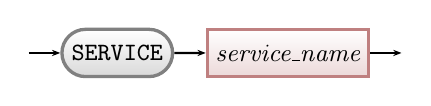
\begin{tikzpicture}[
  start chain=going right,
  node distance=5mm and 4mm,
  every node/.style={on chain},
  every join/.style={rr arrow},
]
  \node[rr point] {};
  \node[rr terminal,join] {SERVICE};
  \node[rr nonterminal,join] {service\_name};
  \node[rr point,join] {};
\end{tikzpicture}

\bigskip

% --- mode_directive ---
\noindent\textbf{mode\_directive}
\medskip

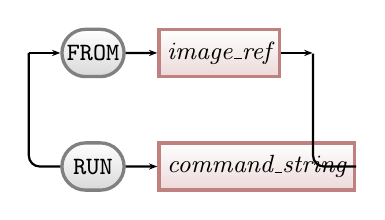
\begin{tikzpicture}[node distance=5mm and 4mm]
  \node[rr point] (start) {};

  \node[rr terminal,right=of start] (from) {FROM};
  \node[rr nonterminal,right=of from] (img) {image\_ref};

  \node[rr terminal,below=8mm of from] (run) {RUN};
  \node[rr nonterminal,right=of run] (cmd) {command\_string};

  \node[rr point,right=of img] (end) {};

  \draw[rr arrow] (start) -- (from);
  \draw[rr arrow] (from) -- (img);
  \draw[rr arrow] (img) -- (end);

  \draw[rr line,rounded corners] (start.east) |- (run.west);
  \draw[rr arrow] (run) -- (cmd);
  \draw[rr line,rounded corners] (cmd.east) -| (end.south);
\end{tikzpicture}

\bigskip

% --- container_directive ---
\noindent\textbf{container\_directive}
\medskip

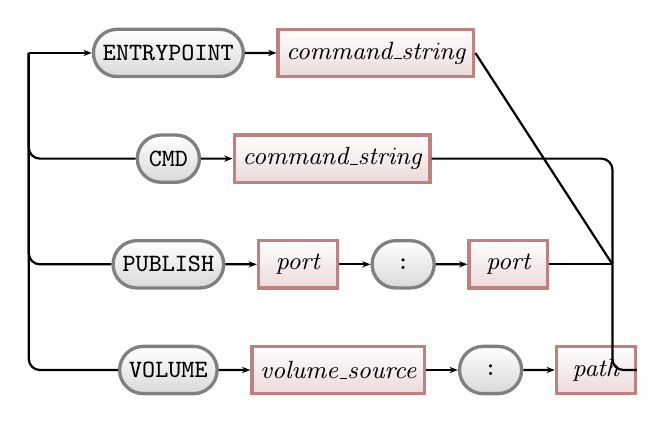
\begin{tikzpicture}[node distance=5mm and 4mm]
  \node[rr point] (start) {};

  \node[rr terminal,right=8mm of start] (ep) {ENTRYPOINT};
  \node[rr nonterminal,right=of ep] (ep_v) {command\_string};

  \node[rr terminal,below=7mm of ep] (cm) {CMD};
  \node[rr nonterminal,right=of cm] (cm_v) {command\_string};

  \node[rr terminal,below=7mm of cm] (pub) {PUBLISH};
  \node[rr nonterminal,right=of pub] (p1) {port};
  \node[rr terminal,right=of p1] (colon) {:};
  \node[rr nonterminal,right=of colon] (p2) {port};

  \node[rr terminal,below=7mm of pub] (vol) {VOLUME};
  \node[rr nonterminal,right=of vol] (vs) {volume\_source};
  \node[rr terminal,right=of vs] (colon2) {:};
  \node[rr nonterminal,right=of colon2] (pa) {path};

  % end point to the right of the longest row
  \node[rr point] (end) at (pa.east -| p2.east) {};
  \coordinate (endx) at ([xshift=8mm]p2.east);
  \node[rr point] (end) at (endx) {};

  \draw[rr arrow] (start) -- (ep);
  \draw[rr arrow] (ep) -- (ep_v);
  \draw[rr line] (ep_v.east) -- (endx);

  \draw[rr line,rounded corners] (start.east) |- (cm.west);
  \draw[rr arrow] (cm) -- (cm_v);
  \draw[rr line,rounded corners] (cm_v.east) -| (endx);

  \draw[rr line,rounded corners] (start.east) |- (pub.west);
  \draw[rr arrow] (pub) -- (p1);
  \draw[rr arrow] (p1) -- (colon);
  \draw[rr arrow] (colon) -- (p2);
  \draw[rr line] (p2.east) -- (endx);

  \draw[rr line,rounded corners] (start.east) |- (vol.west);
  \draw[rr arrow] (vol) -- (vs);
  \draw[rr arrow] (vs) -- (colon2);
  \draw[rr arrow] (colon2) -- (pa);
  \draw[rr line,rounded corners] (pa.east) -| (endx);
\end{tikzpicture}

\bigskip

% --- bool ---
\noindent\textbf{bool}
\medskip

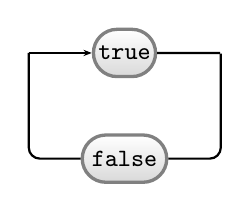
\begin{tikzpicture}[node distance=5mm and 4mm]
  \node[rr point] (start) {};
  \node[rr terminal,right=8mm of start] (t) {true};
  \node[rr terminal,below=7mm of t] (f) {false};
  \node[rr point,right=8mm of t] (end) {};

  \draw[rr arrow] (start) -- (t);
  \draw[rr line] (t) -- (end);
  \draw[rr line,rounded corners] (start.east) |- (f.west);
  \draw[rr line,rounded corners] (f.east) -| (end.south);
\end{tikzpicture}

\bigskip

% --- restart_policy ---
\noindent\textbf{restart\_policy}
\medskip

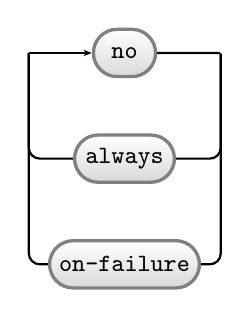
\begin{tikzpicture}[node distance=5mm and 4mm]
  \node[rr point] (start) {};
  \node[rr terminal,right=8mm of start] (a) {no};
  \node[rr terminal,below=7mm of a] (b) {always};
  \node[rr terminal,below=7mm of b] (c) {on-failure};
  \node[rr point,right=8mm of a] (end) {};

  \draw[rr arrow] (start) -- (a);
  \draw[rr line] (a) -- (end);
  \draw[rr line,rounded corners] (start.east) |- (b.west);
  \draw[rr line,rounded corners] (b.east) -| (end.south);
  \draw[rr line,rounded corners] (start.east) |- (c.west);
  \draw[rr line,rounded corners] (c.east) -| (end.south);
\end{tikzpicture}

\bigskip

% --- duration ---
\noindent\textbf{duration}
\medskip

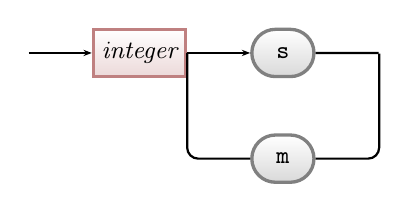
\begin{tikzpicture}[node distance=5mm and 4mm]
  \node[rr point] (start) {};
  \node[rr nonterminal,right=8mm of start] (int) {integer};
  \node[rr terminal,right=8mm of int] (s) {s};
  \node[rr terminal,below=7mm of s] (m) {m};
  \node[rr point,right=8mm of s] (end) {};

  \draw[rr arrow] (start) -- (int);
  \draw[rr arrow] (int) -- (s);
  \draw[rr line] (s) -- (end);
  \draw[rr line,rounded corners] (int.east) |- ([xshift=-4mm]m.west) -- (m.west);
  \draw[rr line,rounded corners] (m.east) -| (end.south);
\end{tikzpicture}

\bigskip

% --- memory_size ---
\noindent\textbf{memory\_size}
\medskip

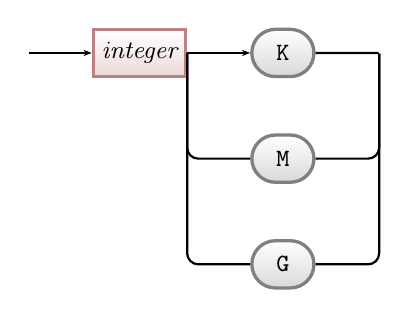
\begin{tikzpicture}[node distance=5mm and 4mm]
  \node[rr point] (start) {};
  \node[rr nonterminal,right=8mm of start] (int) {integer};
  \node[rr terminal,right=8mm of int] (k) {K};
  \node[rr terminal,below=7mm of k] (mb) {M};
  \node[rr terminal,below=7mm of mb] (g) {G};
  \node[rr point,right=8mm of k] (end) {};

  \draw[rr arrow] (start) -- (int);
  \draw[rr arrow] (int) -- (k);
  \draw[rr line] (k) -- (end);
  \draw[rr line,rounded corners] (int.east) |- ([xshift=-4mm]mb.west) -- (mb.west);
  \draw[rr line,rounded corners] (mb.east) -| (end.south);
  \draw[rr line,rounded corners] (int.east) |- ([xshift=-4mm]g.west) -- (g.west);
  \draw[rr line,rounded corners] (g.east) -| (end.south);
\end{tikzpicture}

\bigskip

% --- service_name ---
\noindent\textbf{service\_name} {\small(max 63 characters)}
\medskip

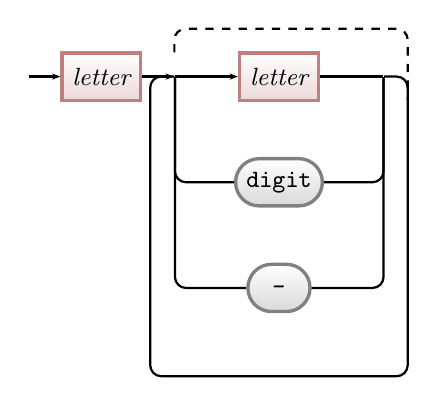
\begin{tikzpicture}[
  start chain=going right,
  node distance=5mm and 4mm,
  every node/.style={on chain},
  every join/.style={rr arrow},
]
  \node[rr point] (start) {};
  \node[rr nonterminal,join] (letter) {letter};
  \node[rr point,join] (mid) {};

  \node[rr nonterminal,right=8mm of mid] (l2) {letter};
  \node[rr terminal,below=7mm of l2] (d) {digit};
  \node[rr terminal,below=7mm of d] (h) {-};

  \node[rr point,right=8mm of l2] (end) {};

  \draw[rr arrow] (mid) -- (l2);
  \draw[rr line] (l2) -- (end);
  \draw[rr line,rounded corners] (mid.east) |- (d.west);
  \draw[rr line,rounded corners] (d.east) -| (end.south);
  \draw[rr line,rounded corners] (mid.east) |- (h.west);
  \draw[rr line,rounded corners] (h.east) -| (end.south);
  \draw[rr line,rounded corners] (end.east) -- ++(0.3,0) |- ([yshift=-8mm]h.south) -| ([xshift=-3mm]mid.west) -- (mid.west);

  \draw[rr line,dashed,rounded corners] (mid.north) ++ (0,3mm) -- ++(0,3mm) -| ([xshift=3mm]end.east) -- ++ (0,-3mm);
\end{tikzpicture}

\bigskip

% --- var_ref ---
\noindent\textbf{var\_ref}
\medskip

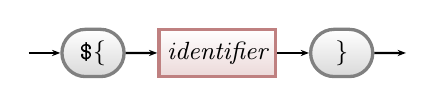
\begin{tikzpicture}[
  start chain=going right,
  node distance=5mm and 4mm,
  every node/.style={on chain},
  every join/.style={rr arrow},
]
  \node[rr point] {};
  \node[rr terminal,join] {\$\{};
  \node[rr nonterminal,join] {identifier};
  \node[rr terminal,join] {\}};
  \node[rr point,join] {};
\end{tikzpicture}

% --- clear_directive ---
\noindent\textbf{clear\_directive}
\medskip

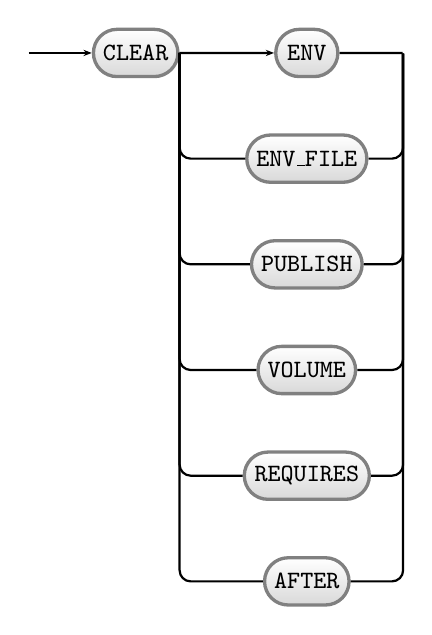
\begin{tikzpicture}[node distance=5mm and 4mm]
  \node[rr point] (start) {};
  \node[rr terminal,right=8mm of start] (clear) {CLEAR};

  \node[rr terminal,right=12mm of clear] (env) {ENV};
  \node[rr terminal,below=7mm of env] (envf) {ENV\_FILE};
  \node[rr terminal,below=7mm of envf] (pub) {PUBLISH};
  \node[rr terminal,below=7mm of pub] (vol) {VOLUME};
  \node[rr terminal,below=7mm of vol] (req) {REQUIRES};
  \node[rr terminal,below=7mm of req] (aft) {AFTER};

  \node[rr point,right=8mm of env] (end) {};

  \draw[rr arrow] (start) -- (clear);
  \draw[rr arrow] (clear) -- (env);
  \draw[rr line] (env) -- (end);

  \draw[rr line,rounded corners] (clear.east) |- (envf.west);
  \draw[rr line,rounded corners] (envf.east) -| (end.south);
  \draw[rr line,rounded corners] (clear.east) |- (pub.west);
  \draw[rr line,rounded corners] (pub.east) -| (end.south);
  \draw[rr line,rounded corners] (clear.east) |- (vol.west);
  \draw[rr line,rounded corners] (vol.east) -| (end.south);
  \draw[rr line,rounded corners] (clear.east) |- (req.west);
  \draw[rr line,rounded corners] (req.east) -| (end.south);
  \draw[rr line,rounded corners] (clear.east) |- (aft.west);
  \draw[rr line,rounded corners] (aft.east) -| (end.south);
\end{tikzpicture}

\bigskip

% ============================================================================
\newpage
\section{Constraints}
% ============================================================================

The following constraints are enforced by the parser and cannot be expressed
in the EBNF grammar alone:

\begin{description}
  \item[C1: FROM XOR RUN] A service must specify exactly one of \texttt{FROM}
    (container mode) or \texttt{RUN} (host mode). Both or neither is an error.

  \item[C2: Container-only directives] \texttt{ENTRYPOINT}, \texttt{CMD},
    \texttt{PUBLISH}, \texttt{VOLUME} are only valid with \texttt{FROM}.

  \item[C3: Host-only directives] \texttt{USER}, \texttt{STOP},
    \texttt{RELOAD} are only valid with \texttt{RUN}.

  \item[C4: Dependency acyclicity] \texttt{REQUIRES} and \texttt{AFTER}
    edges must form a directed acyclic graph (DAG). Cycles are a parse error.
\end{description}

\end{document}
